\noindent
\begin{tabular}{cc}
\begin{minipage}[b]{0.60\textwidth}
\begin{exerciseS}[Corrente in canale aperto]
Si consideri il flusso d'acqua, $\overline{\rho}=999\ kg/m^3$, 
nel canale rappresentato in figura.
Nel primo tratto l'acqua scorre con una velocit\`{a} uniforme 
$U_1 = 1\ m/s$  e l'altezza del pelo libero rispetto al fondo 
del canale \`e $h_1 = 1.5\ m$. Determinare la velocit\`{a}
dell'acqua $U_2$ e l'altezza del pelo libero $h_2$ nel secondo tratto 
del canale, sapendo che l'altezza del fondo del primo tratto rispetto al fondo
del secondo tratto \`{e} $H=0.5\ m$. Si trascuri qualunque effetto
dissipativo.

(Soluzione 1: $U_2 = 0.741\ m/s$, $h_2 = 2.022\ m$.
Soluzione 2: $U_2 = 5.940\ m/s$, $h_2 = 0.252\ m$)
\end{exerciseS}
\end{minipage}
&
\begin{minipage}{0.35\textwidth}
   \begin{center}
   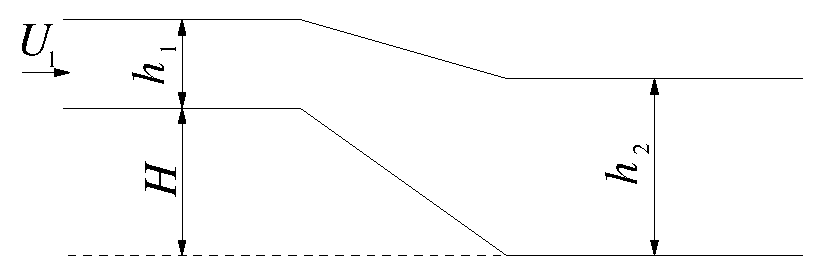
\includegraphics[width=0.90\textwidth]{./fig/canale.eps}
   \end{center}
\end{minipage}
\end{tabular}

\sol

\partone
Teorema di Bernoulli nel caso incomprimibile, non viscoso, stazionario, irrotazionale.
Soluzione di equazioni di terzo grado: metodo grafico e numerico. 
Correnti in canali aperti: soluzioni ``fisiche'', numero di Froude $Fr$,
 correnti subrcritiche e supercritiche.

\parttwo

L'esercizio viene risolto in due passi, che richiedono diversi livelli di
 conoscenza della dinamica dei fluidi in canali aperti: in un primo tempo,
 vengono ricavate le soluzioni ammissibili ($h_2 > 0$, $U_2 > 0$) del 
 problema; in un secondo tempo, viene scelta la soluzione fisica del
 problema, tra le due soluzioni ammissibili trovate in precedenza.

\paragraph{Parte 1.}
L'esercizio viene risolto mettendo a sistema il teorema di Bernoulli riferito
 a una linea di corrente sul pelo libero
(sul quale agisce la pressione ambiente $P_a$, costante) e l'equazione di
 continuità.
Grazie alle ipotesi elencate in precedenza, si può scrivere il sistema risolvente come:

\begin{equation}\label{eqn:bern_cont}
  \begin{cases}
    \frac{1}{2}\rho U_1^2 + \rho g(h_1+H) = \frac{1}{2}\rho U_2^2 +
    \rho g h_2 \\
    h_1 U_1 = h_2 U_2
  \end{cases}
\end{equation}

Il sistema è di due equazioni (non lineari) nelle incognite $U_2$ e $h_2$. Se si ricava una delle due incognite
da un'equazione e la si inserisce nell'altra, si ottiene un'equazione di terzo grado. Per esempio, ricavando $h_2$ 
dalla prima e inserendola nella seconda, per l'incognita $U_2$ si ottiene l'equazione di terzo grado:

\begin{equation}
  h_1 U_1 = U_2 \displaystyle\left( \frac{U_1^2 - U_2^2}{2 g} + (h_1 + H)    \right)
\end{equation}


I metodi numerici convergono (quando convergono) a una soluzione, senza informazioni su quante soluzioni
esistono effettivamente: prima di risolvere l'equazione di terzo grado con un
 metodo numerico è utile un primo approccio analitico al problema. 

Per questo cerchiamo le soluzioni del sistema di due equazioni per via grafica. Le equazioni del sistema \ref{eqn:bern_cont}
 definiscono curve nel piano $(U_2,h_2)$. Se scegliamo di usare come asse orizzontale quello delle $U_2$, la prima equazione definisce una parabola con la concavità diretta verso il basso ($h_2 = - 0.5  U_2^2 /g +...$), mentre la seconda un'iperbole.
 
\begin{center}
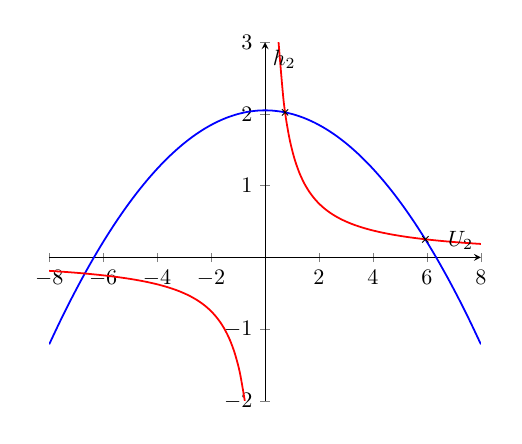
\begin{tikzpicture}[scale=0.80]
\begin{axis}[axis lines=middle, domain=-8.0:8.0, xlabel={$U_2$}, ylabel={$h_2$}]
\addplot
[domain=-8:8,samples=40,smooth,thick,blue]
{-0.5/9.81 * x^2 + 2.05};
\addplot
[domain=-8:-0.75,samples=40,smooth,thick,red]
{1.5/x};
\addplot
[domain=0.5:8,samples=40,smooth,thick,red]
{1.5/x};
\addplot[color=black,mark=x] coordinates{
         (0.741, 2.022)};
\addplot[color=black,mark=x] coordinates{         
         (5.940, 0.252)};
%\legend{$f_1(x)$,$\frac{\rho_s}{\rho}=0.842$}
\end{axis}
\end{tikzpicture}
\end{center}

Esistono due soluzioni con senso fisico ($h_2 \ge 0, U_2 \ge 0$). Ora che sappiamo quante soluzioni cercare e dove cercarle, possiamo procedere con un metodo numerico, dando guess iniziali in un intorno della soluzione.
Le due soluzioni sono:
\begin{equation}
\begin{aligned}
  A :
  \begin{cases}
   U_2 = 0.741 \ m/s \\
   h_2 = 2.022 \ m
  \end{cases}
   \quad
  B :
  \begin{cases}
   U_2 = 5.940 \ m/s \\
   h_2 = 0.252 \ m
  \end{cases}
\end{aligned}
\end{equation}

\paragraph{Parte 2.}
\'E plausibile farsi una domanda: al netto delle ipotesi fatte sul regime di
 moto (fluido incomprimibile, non viscoso), il modello è in grado di
 descrivere il fenomeno fisico e stabilire quale delle due soluzioni 
 amissibili trovate è la soluzione ``fisica''?
Seguendo la trattazione del problema svolta in \href{http://heidarpour.iut.ac.ir/sites/heidarpour.iut.ac.ir/files//u32/open-chaudhry.pdf}{Chaudhry, \textit{Open-Channel Flow}, paragrafo 2-7: Channel transition e paragrafi vicini},
 è possibile trovare l'unica soluzione fisica del problema.
 Viene introdotta la notazione usata da Chaudhry, che contrasta in parte
 con quella usata finora. Si tornerà alla notazione usata nella prima parte
 dell'esercizio, solo alla fine per scrivere i risultati.

La variabile
 $z(x)$ descrive la quota del fondo del canale, la variabile $y(x)$ descrive
 la profondità della corrente, riferita al fondo del canale. Si indica
 con $Q = V y $ la portata in volume, costante.
Il trinomio di Bernoulli $H$, diviso per $\rho$ e $g$, è costante lungo il
 canale. Si ricorda che sulla linea di corrente in corrispondenza del pelo
 libero agisce una pressione costante uguale alla pressione ambiente $P_a$.
Se si introduce la coordinata orizzontale $x$,
\begin{equation}
\begin{aligned}
 0 = \dfrac{d H}{d x} = 
 & \dfrac{d (y+z)}{d x} + \dfrac{d}{d x} \dfrac{V^2}{2 g}     = \\
 & = \dfrac{d (y+z)}{d x} + \dfrac{d}{d x} \dfrac{Q^2}{2 g y^2} = \\
 & = \dfrac{d (y+z)}{d x} - \dfrac{Q^2}{g y^3} \dfrac{d y}{d x} = \\
 & = \dfrac{d (y+z)}{d x} - \dfrac{V^2}{g y} \dfrac{d y}{d x} = \\ 
 & = \dfrac{d (y+z)}{d x} - \text{Fr}^2 \dfrac{d y}{d x} = \\ 
 & = \dfrac{d z}{d x} - (\text{Fr}^2 - 1) \dfrac{d y}{d x} \\ 
\end{aligned}
\end{equation}
dove è stato introdotto il numero di Froude $\textit{Fr} = V(y)^2 / g y$, e
 qui è stata esplicitata la dipendenza dalla profondità $y$, funzione a sua
 volta funzione della coordinata $x$.
Si trova così il legame tra la profondità della corrente $y(x)$, la quota
 del fondo $z(x)$ e lo stato della corrente, descritto dal numero di Froude.
\begin{equation}\label{eqn:flow_depth}
 \dfrac{d z}{d x} = (\text{Fr}^2(y(x)) - 1) \dfrac{d y}{d x}
\end{equation}
Vengono definiti due regimi di moto: subcritico $\textit{Fr} < 1$,
 supercritico $\textit{Fr} > 1$. Il profilo del fondo $z(x)$,
 e quindi la sua derivata, è noto dal progetto del canale.
 La profondità della corrente $y(x)$ può essere ottenuta integrando l'eq.
 \ref{eqn:flow_depth} con le condizioni iniziali note sulla sezione di 
 ingresso.

Per risolvere il nostro esercizio è sufficiente ragionare sui segni dei tre
 termini dell'eq. \ref{eqn:flow_depth}: $dz/dx \le 0$, quindi i due fattori
 alla destra dell'uguale devono essere discordi.
Il numero di Froude sulla sezione di ingresso del problema vale
 $\text{Fr}_1 = U^2_1 / (g h_1) = 0.068$, quindi il contenuto della parentesi
 tonda è negativo (e negativo rimane, al variare di $x$; di questo dovete
 fidarvi...).
 Deve quindi essere $dy/dx \ge 0$. Tornando alla notazione usata nella prima
 parte dell'esercizio, dove la profondità della corrente è indicata con
 $h(x)$, $dh(x)/dx \ge 0$. Poichè la profondità della corrente aumenta
 sempre, la soluzione ``fisica'' tra le due ammissibili è la soluzione $A$,
 per la quale $h_2 > h_1$.

\begin{equation}
  \begin{cases}
   U_2 = 0.741 \ m/s \\
   h_2 = 2.022 \ m
  \end{cases}
\end{equation}

\vspace{0.5cm}
\paragraph{Cosa non è stato detto.} \'E stato fatto solo un accenno al 
 ragionamento che consente di determinare l'unica soluzione ``fisica'' del
 problema delle correnti in canali aperti che variano con continuità.
 Non si dirà nulla sui salti idraulici (che portano la corrente da uno
 stato supercritico a uno subcritico), dei quali si possono trovare 
 esempi nei fiumi o sul fondo di un lavandino.
Si accenna solo alla uguaglianza formale del problema del moto
 di un fluido incomprimibile in un canale aperto, con il moto
 monodimensionale di un 
 fluido comprimibile, dove il ruolo del numero di Froude $\textit{Fr}$
 sarà svolto dal numero di Mach $M$, la definizione di stato sub- e
 supercritico, sarà sostituita da quella di condizione sub- e supersonica,
 il salto idraulico troverà il suo fenomeno corrispondente nelle onde d'urto.
